\section{Methodology}

\subsection{Centralized state}
La realizzazione del sistema \`e stata effettuata utilizzando alcune tra le tecnologie ed i pattern pi\`u in auge nello sviluppo di applicazioni web-oriented. Nello specifico sono stati utilizzati i pattern Unidirectional Data Flow e Immutability attraverso l'implementazione messa a disposizione rispettivamente dalle librerie ReduxJS e ImmutableJS.


Lo sviluppo del progetto si \`e focalizzato sull'individuazione di una struttura gerarchica in grado di rappresentare in modo esaustivo l'insieme delle componenti che compongono la planimetria, costituendo di fatto lo stato dell'applicazione. Lo stato \`e stato gestito attraverso l'immutabilit\`a, un principio che prevede l'applicazione di nuove modifiche attraverso la generazione di un nuovo stato, in primis identico al precedente, ma sul quale vengono applicate le modifiche richieste. Dal punto di vista della gestione della memoria questo meccanismo richiederebbe un importante dispendio di risorse. Per evitare ci\`o l'implementazione ImmutableJS adotta dei meccanismi che simulano il principio di immutabilit\`a evitando la copia in profondit\`a della memoria  (deep clone) e alleggerendo cos\`i il carico in termini di utilizzo di memoria e tempo macchina.


\subsubsection{Application as Finite State Machine}
Per dominare la complessit\`a dell'applicazione l'intero sistema \`e stato modellato su una macchina a stati. Sfruttando il modello basato su azioni e reducer messo a disposizione dal pattern unidirectional data flow \`e stato individuato un grafo che rappresenta le possibili evoluzioni dello stato dell'applicazione. Ogni nodo corrisponde ad una modalit\`a, ogni arco corrisponde alle possibili azioni che è possibile intraprendere a partire da quel punto. A seconda della modalit\`a gli eventi del browser, come ad esempio \texttt{click} o \texttt{mousemove}, vengono mappati sulle azioni.

\begin{figure}[!t]
\centering
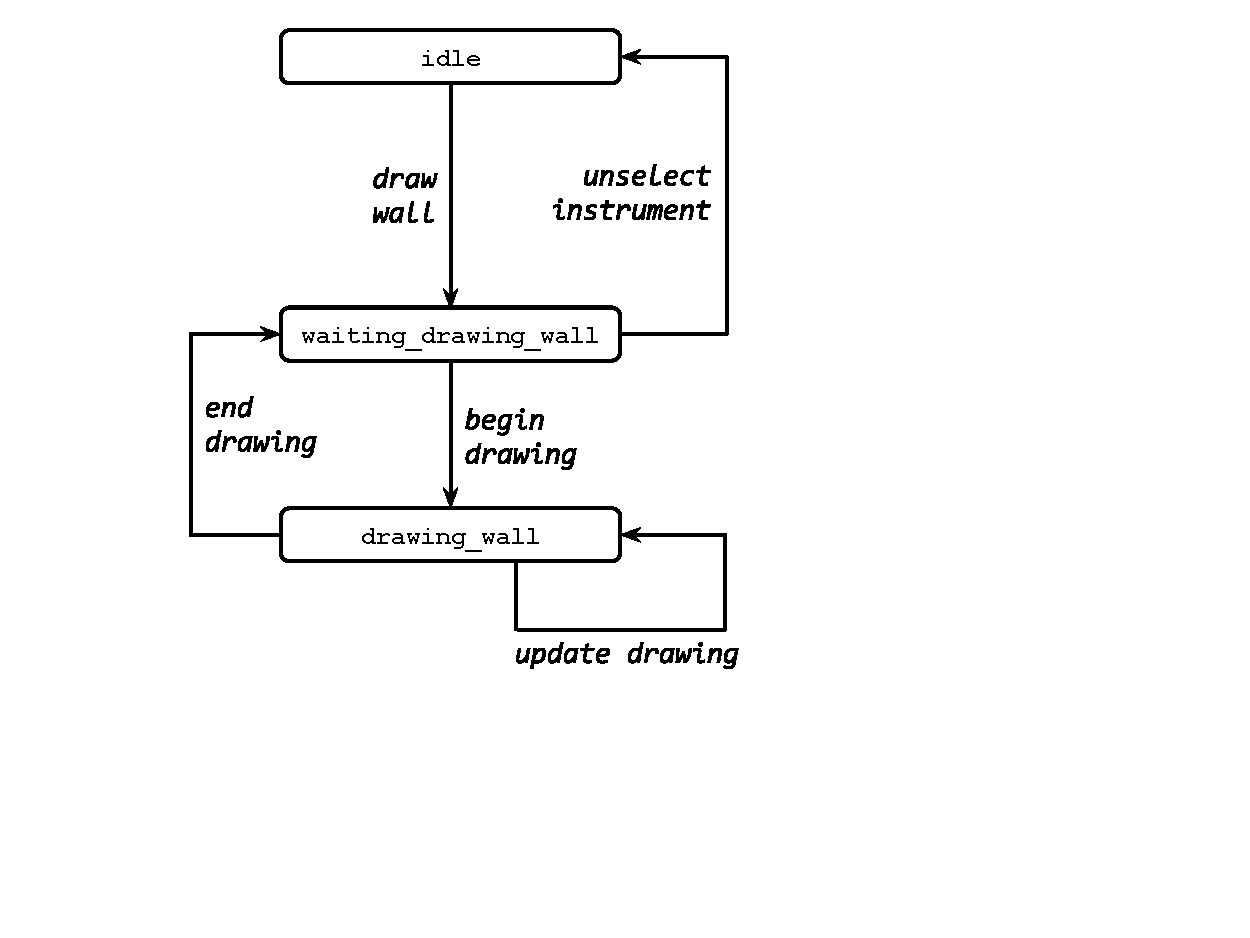
\includegraphics[width=\linewidth]{contents/images/uc_draw_wall}

\caption{Sottografo della macchina a stati che rappresenta la creazione di un muro. (i) Nodo \texttt{idle}: modalit\'a d'attesa dell'applicazione. Non è stata ancora intrapresa nessuna operazione. (ii) Nodo \texttt{waiting\_drawing\_wall}: l'utente ha selezionato lo strumento disegno muro, ma non ha ancora iniziato il disegno. (iii) Nodo \texttt{drawing\_wall}: l'utente ha posizionato il punto di inizio del muro.}
\label{fig_sim}
\end{figure}




\subsection{Collaboration}
    Per permettere all'utente finale di gestire parti di edificio si \`e introdotto un concetto di layer, un raggruppamento di elementi accomunati da caratteristiche di similarit\`a decise dall'utente. Un esempio potrebbe essere l'intero piano di una palazzina oppure un'area di un edificio. La gestione collaborativa del progetto sfrutta questi layer per permettere a pi\`u persone di operare contemporaneamnte grazie a dei lock che abilitano la modifica su layer ad una persona per volta. In questo modo gli utenti possono lavorare contemporaneamente su pi\`u layer evitando conflitti a livello di progetto.


\subsection{Building elements}

L'insieme degli elementi che \`e possibile inserire all'interno della planimetria vengono gestiti in un catalogo, strutturato in categorie.
La categorizzazione individua un insieme di casi d'uso con cui l'utente pu\`o interagire.

\textbf{Walls}, rientrano in questa categoria tutti i tipi di muro (perimetrali, interni, portanti). La creazione avviene specificando il punto di inizio e fine dell'elemento. La rappresentazione interna viene ricondotta a quella di un grafo in cui: i \textbf{nodi} corrispondono ai punti geometrici in cui si intersecano pi\`u muri e hanno delle coordinate che li collocano nello spazio; gli \textbf{archi} corrispondono al muro.\\
\textbf{Openings}, rientrano in questa categoria gli elementi che bucano i muri come porte, finestre e archi. La creazione viene effettuata attraverso uno snap sui muri precedentemente creati. La rappresentazione interna associa ciascuna apertura con il muro di riferimento, creando un legame tra le due componenti.\\
\textbf{Areas}, rientrano in questa categoria i pavimenti. La creazione viene effettuata automaticamente attraverso un'analisi del grafo composto dai muri. L'algoritmo individuato si compone delle seguenti fasi:\\
    - Ricerca delle componenti biconnesse attraverso l'applicazione dell'algoritmo Hopcroft-Tarjan [Citazione]
    - Rimozione degli archi che non appartengono alle componenti biconnesse
    - Applicazione dell'algoritmo di ricerca del bordo per la determinazione dei cicli [Citazione]
    - Rimozione del ciclo massimale, corrispondente ad un ciclo che coinvolge tutti gli archi perimetrali del grafo attraverso la legge.... [Citazione]

\textbf{Objects}, rientrano in questa categoria tutti gli oggetti posizionabili sulle aree. L'utente pu\`o agire sulla disposizione sia in termini di posizione che rotazione.\\

\subsection{UI components}

L'intera applicazione \`e stata pensata in maniera modulare, in modo da poterla estendere in maniera semplice. Dal punto di vista web la tecnologia applicata \`e stata quella dei \textbf{Web Components}. L'idea di base \`e quello di definire l'applicazione frontend come una collezione di componenti, che vengono renderizzati in modo diverso a seconda dei valori assegnati allo stato. In particolare, vi \`e una classe di componenti delegati alla rappresentazione delle propriet\`a dello stato stesso: i \textbf{viewers}. Esempi sono i visualizzatori per il 2D e per il 3D. In generale, la struttura a componenti permette di definire una qualunque visualizzazione dello stato (ad esempio in forma tabellare) semplicemente inserendo un nuovo componente. Una schematizzazione del concetto \`e evidenziata nella figura~\ref{fig_viewers}.\\

Come possiamo vedere nello schema, siamo in grado di identificare tre macro blocchi. Il primo \`e il catalogo, che come abbiamo visto (CITAZIONE AL PARAGRAFO) contiene tutti i building elements del sistema e le loro properiet\`a. Il secondo \`e il core vero e proprio e si occupa della gestione dello stato e contiene le funzionalit\`a di disegno. Questo comunica con il catalogo prendendo le propriet\`a dei building elements. Infine abbiamo i visualizzatori veri e propri, che vengono scelti in base alla \texttt{mode} property inside the state.\\

Al momento sono stati implementati i visualizzatori 2D e 3D.\\\\
\textbf{2D Viewer}. This viewer creates a 2D view of the building model. Dato lo stato globale, \`e in grado di sfruttare il \textbf{Virtual DOM} per aggiornare solo le parti che vengono modificate evitando aggiornamenti globali continui\\\\
\textbf{3D Viewer}. Sfrutta la libreria di modellazione per WebGL \textbf{ThreeJS} per creare una vista 3D del building model. Per evitare di dover continuamente ricreare l'intero modello quando cambiano porzioni dello stato, \`e stato implementato un sistema di \textit{diff} e \textit{patch} dello stato (usando la libreria \texttt{immutable-js-diff}) che a sua volta si riconduce allo stato citato in~\cite{rfc6902}. In pratica \`e stata creata una struttura parallela che mappa gli oggetti di ThreeJS con i relativi building elements memorizzati nello stato. Ogni volta che viene lanciata un'azione redux, viene calcolata la diff tra il vecchio stato e quello nuovo e si ricreano solo gli oggetti che sono stati modificati. In particolare possiamo avere tre possibili \textit{operations}: (i) \textbf{add}, (ii) \textbf{replace} and (iii) \textbf{remove}. For every operation, viene determinato un diverso tipo di comportamento in base al particolare building element cambiato, coinvolgendo eventualmente building elements correlati

\begin{figure}[!t]
\centering
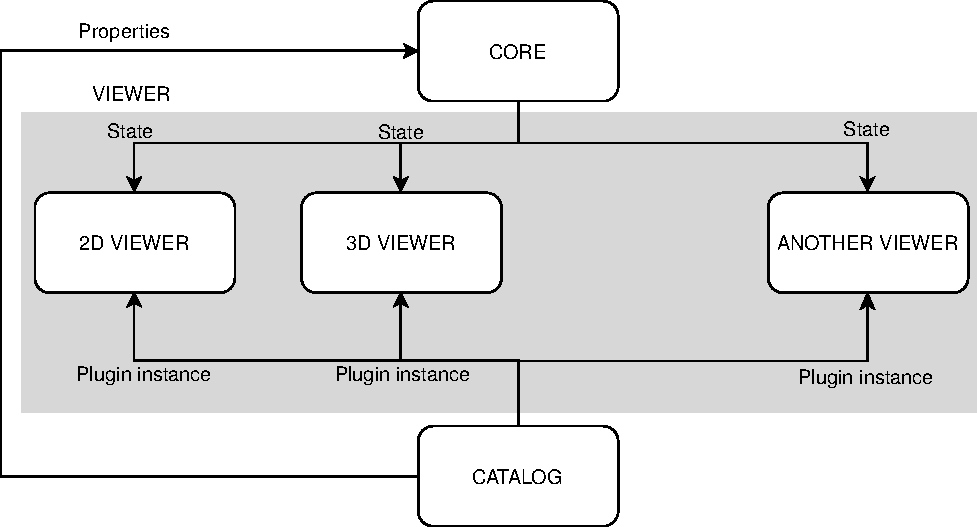
\includegraphics[width=\linewidth]{contents/images/diagramma-visualizzatori}

\caption{The architectural schema for the viewers. Here we can see that the core can instanziate several different viewers giving them the state for the representation}
\label{fig_viewers}
\end{figure}

\subsection{Architettura serverless}
Una tra le sfide che ha caratterizzato il progetto \`e l'utilizzo di un approccio serverless. L'intera applicazione viene eseguita all'interno del browser, ottenendo i vantaggi di: (i) evitare all'utilizzatore complicate installazioni del sistema o procedure di aggiornamento; (ii) fornire un livello di astrazione tale da rendere l'ambiente compatibile su diverse macchine e su diversi sistemi operativi; (iii) abilitare un rilascio di nuove versioni centralizzato, in grado di raggiungere tutti gli utenti contemporanemante; (iv) eliminare il punto di concentramento del calcolo in quanto questo rimane confinato sulla macchina dell'utente.
Per permettere la generazione di elementi architetturali complessi il sistema \`e in grado inoltre di sfruttare dei worker di tipo FaaS (Function as a Service) demandando l'onerosa generazione delle geometrie 3D necessarie alla visualizzazione.